\documentclass[a4paper]{article}



\usepackage{amsmath}
\usepackage[version=3]{mhchem}
\usepackage{booktabs}
\usepackage{xcolor,graphicx}
%plotting
\usepackage{tikz}
\usepackage{csvsimple}
\usepackage{tikzscale}
\usepackage{pgfplots, pgfplotstable}
\usepgfplotslibrary{statistics}
\pgfplotsset{compat=1.7}

%Spacing between paragraphs
\setlength{\parskip}{\baselineskip}%
%No indent
\setlength{\parindent}{0pt}

%%%%%%%%%%%%%%%%%%%%%%%%%%%%%%%%%%%%%%%%%%%%%%%%%%%%%%%%%%%

\begin{document}

\title{Getting started with LaTeX}
\author{You \and Me}
\date{\today}
\maketitle

\tableofcontents

\section{Title of the First Section}
... text ... 
\subsection{Title of the First Subsection}
... text ... 
\subsubsection{Title of the First Subsubsection}
... text ... 
\subsubsection*{Title of the Second Subsubsection} 
\addcontentsline{toc}{subsubsection}{Something Else} 

\newpage
There are two main ways to create lists in LaTeX, enumerate (for numbered lists) 
and itemize. Here is an example using enumerate 

%As always we have to start the environment 
\begin{enumerate}
%Add items to the list via \item
\item This is a thing
\item This is another thing 
\end{enumerate}

The lists don't have to be numbered. Using itemize will give you bullet points 
(but you can change what they are). 
\begin{itemize}
%Again we add items to the list with \item 
\item Stuff
\item More stuff 
\end{itemize}

\newpage
One of the primary reasons you will use \LaTeX \ is for writing equations.  

\begin{equation}
F_{net}=ma
\end{equation}

Equations don't have to be numbered. You can disable the numbering by putting 
an asterisk in the begin and end statements 
\begin{equation*}
E=mc^{2}
\end{equation*}
It is also very convenient to write multiple lines in an equation using 
the align environment:
\begin{align*}
2x - 5y &=  8 \\ 
3x + 9y &=  -12
\end{align*}
You can write all sorts of fancy symbols (which can be found on the cheatsheet!)
\begin{equation*}
i\hbar \frac{\partial | \Psi \rangle}{ \partial t}=\hat{H}|\Psi \rangle
\end{equation*}
\newpage

Math mode can be used inline with text (e.g. $e^{-\lambda x}$) which is very 
convenient. All you need to do is wrap your equation (or whatever you are using)
in dollar signs. 


Making pretty looking chemistry equations:

\ce{CO2+C -> 2CO2}

\newpage


Here we will create tables which can be a nice way of presenting data. 

%Begin the tabular environment 
\begin{center}
%The c's indicate center justified text
%Vertical lines will put vertical lines between columns 
\begin{tabular} { c  c  c }
\toprule
Fruit & Quantity & Price \\ \midrule
Apple & 2 & \$2.00 \\ \midrule
Banana & 5 & \$3.50 \\ \midrule
Orange & 8 & \$4.00 \\ 
\bottomrule

\end{tabular}
\end{center}

\newpage

%As always we have to start the environment 
\begin{figure}[h]
%This is how we can center the figure 
\begin{center}
%You can resize the figure using the scale option
%There are options to clip the figure as well 
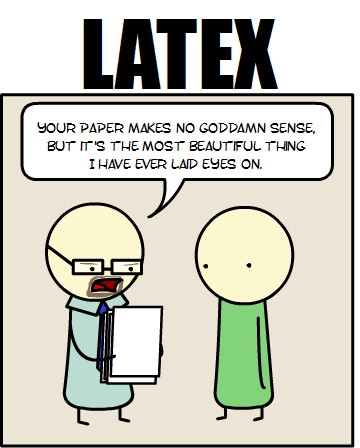
\includegraphics[scale=0.5]{figure_example}
\end{center}
%Add your caption here 
\caption{We can add captions to our figures as well}
%Close the environment 
\end{figure}

\newpage


We can do all kinds of things with text. You can make text \textbf{bold}, 
\emph{italicized}, and \textcolor{blue}{coloured}. In addition it is also 
useful to know how to superscript text A${}^{\text{stuff}}$ or subscript 
B${}_{\text{stuff}}$. 

\newpage

This is a citation \cite{greenwade93}. You will probably need to compile twice to get the reference to show up. 

\bibliographystyle{plain}
\bibliography{ExamplecodeBibTeX.bib}

\newpage

Plotting from a csv file made easy:

\begin{figure}[hb]
\centering
\begin{tikzpicture} 
\begin{semilogyaxis}[
		grid=major,
		width=\textwidth,
		height=8cm,
		title={Uncalibrated Gamma Spectrum},
 		xlabel={channel},
 		xmin=0,
 		xmax=450,
 		xtick={50,100,150,200,250,300,350,400},
 		ylabel={Counts}],
\addplot[only marks, mark size=1pt] table [col sep = comma]{spectrum.csv};	
\end{semilogyaxis} 
\end{tikzpicture}
\caption{The uncalibrated gamma spectrum (raw data from the MCA). Peak channel numbers will be used with the known peak energies to create a calibration curve.}
\end{figure}



You can also plot datapoints directly:

\begin{figure}[h!]
\centering
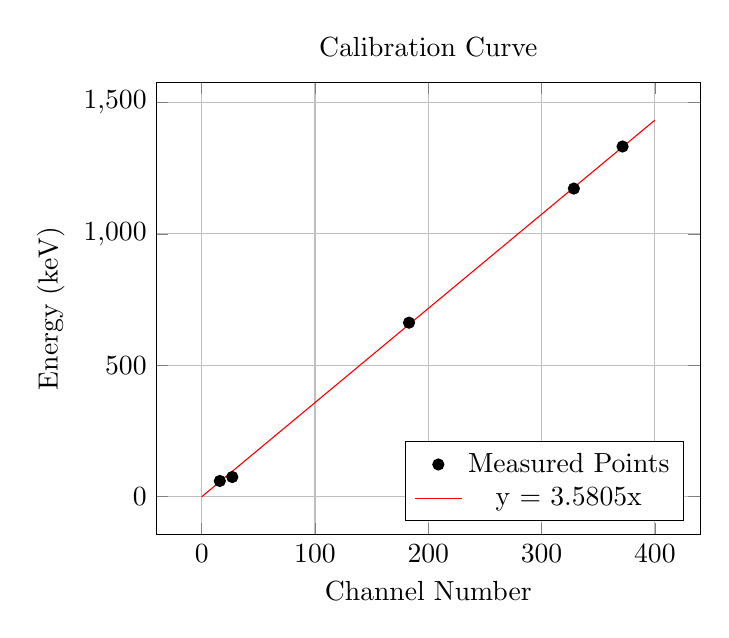
\begin{tikzpicture}

\begin{axis}[
	grid=major,
	legend pos=south east,
	width=0.7\textwidth,
	title={Calibration Curve},
	xlabel={Channel Number},
	ylabel={Energy (keV)},	]
\addplot[only marks] coordinates {
	(16,60)
	(27,75)
	(183,662)
	(328.5,1172)
	(371.5,1332) };
\addlegendentry{Measured Points}
\addplot[draw=red][domain=0:400]{3.5805*x}; \addlegendentry{y = 3.5805x}
\end{axis}
\end{tikzpicture}
\caption{The calibration curve produced from the three sources used in this experiment.}
\end{figure}


\end{document}
